\newpage

\section{Broader Impact}

This work studies a general method for efficient image generation and does not introduce a domain-specific deployment. Potential benefits include lower inference cost and simpler latent-to-pixel generation pipelines, which may make high-quality synthesis more accessible for research and creative applications. At the same time, the method inherits standard risks of image generation systems, including the creation of misleading or harmful synthetic content and the reproduction of biases present in the training data. We therefore expect deployment to require the same safeguards as other generative image models, such as data curation, provenance or watermarking mechanisms, content filtering, and application-specific human oversight.

\section{Implementation Details}
\label{app:implementation_details}

This appendix provides implementation details that are useful for reproduction but not required to understand the main method. The main text summarizes the model design and the role of the auxiliary losses.

\subsection{Compute and Software}

All experiments are conducted on 8 Linux nodes, each with 8 NVIDIA H20 GPUs. Our implementation is based on PyTorch~\citep{pytorch}, Transformers~\citep{transformers_lib}, and timm~\citep{timm_lib}. We use torch-fidelity~\citep{torch_fid_lib} for FID computation. Training uses PyTorch Distributed Data Parallel with a per-GPU batch size of 32. We use the same fixed hyperparameter set across experiments rather than dense hyperparameter tuning.

\subsection{Architecture and Conditioning}

We use the VA-VAE encoder~\citep{VAVAE} as the fixed image encoder and a standard ViT backbone~\citep{ViT} as the CrossFlow generator. On ImageNet $256\times256$, the generator outputs $16\times16$ image patches, giving 256 image patch tokens. We additionally use 16 context tokens for class and time conditioning.

The theoretical formulation permits conditioning on both $t$ and $r$. In the implementation, we condition only on $r$. This choice follows the observation that a model can infer the noise level $t$ from the noisy latent input~\citep{DiffNoTime}, and it keeps the input format the same for reconstruction and one-step generation. Table~\ref{tab:ablation} reports the corresponding ablation: using both $(r,t)$ gives 2.73 FID, while the default $r$-only conditioning gives 2.54 FID.
\begin{center}
\captionof{table}{\textbf{Training setup for CrossFlow variants on ImageNet $256\times256$.} All variants use the same training schedule and differ mainly in depth, hidden dimension, and parameter count.}
\vspace{0.5em}
\small
\begin{tabular}{l c c c}
\toprule
\textbf{Hyperparameter} & \textbf{CrossFlow-B} & \textbf{CrossFlow-L}  & \textbf{CrossFlow-XL} \\
\midrule
Depth (layers) & 12 & 24 & 28\\
Hidden dimension & 768 & 1024 & 1152 \\
\# parameters & 95M & 315M & 461M\\
Patch size & 16 & 16  & 16 \\
\midrule
Epochs & 160 & 160 & 160 \\
Batch size & 2048 & 2048 & 2048 \\
Optimizer & Muon & Muon & Muon \\
Learning rate & 8e-4 & 8e-4 & 8e-4 \\
LR warmup & 5 epochs & 5 epochs & 5 epochs \\
EMA decay & \multicolumn{3}{c}{selected from 0.999/0.9995/0.9999} \\
Weight decay & 1e-6 & 1e-6 & 1e-6 \\
\bottomrule
\end{tabular}
\label{tab:hyperparams}
\end{center}


\subsection{Time Sampling}

For the time distribution, we start from a uniform distribution on $[0,1]$ and apply the shifted-time transformation used in RAE~\citep{RAE},
\begin{equation}
    t \mapsto \frac{\alpha t}{1 + (\alpha - 1)t},
    \qquad
    \alpha = \sqrt{\text{latent dimension}/4096}.
\end{equation}
This transformation adjusts the effective time distribution for different latent dimensionalities. With 50\% probability, we set $t=r$, in which case the CrossFlow loss reduces to the reconstruction endpoint. With the remaining 50\% probability, we sample two shifted times independently and assign them to $t$ and $r$ according to the time ordering used by the training objective.

\subsection{Auxiliary Pixel-Space Losses}

To improve perceptual quality, we combine the CrossFlow objective with perceptual and GAN losses following common VAE training practice~\citep{vqgan}. The perceptual loss is applied to the same scaled prediction and target used in the reconstruction-compatible objective:
\begin{equation}
\mathcal{L}_{\mathrm{perc}} =
\mathrm{PerceptualLoss}\!\left(
\hat{x} + \frac{\bigl(\beta(t)-\beta(r)\bigr)\beta(t)}{\dot{\beta}(t)\beta(r)}\,
\frac{d\hat{x}}{dt},
\Bigl[ \alpha(t) - \frac{\beta(t)}{\dot{\beta}(t)}\dot{\alpha}(t) \Bigr] x_0
\right).
\end{equation}

For adversarial training, we use a hinge GAN objective. The generator loss is
\begin{equation}
    \mathbb E_{t\sim T, z_t\sim p_t} -w(t)D(G(z_t, r)),
\end{equation}
and the discriminator loss is
\begin{equation}
    \mathbb E_{t\sim T, z_t\sim p_t, x\sim p}
    \max(1 - D(G(z_t, r)), 0) + \max(1 + D(x), 0).
\end{equation}
Here $w(t)$ controls the relative adversarial strength across time.

For the GAN discriminator architecture, we use the same architecture as dinoGAN in RAE~\citep{RAE}. For the perceptual loss, we map images to DINOv3-B features~\citep{dinov3} and compute a Huber loss between the feature tensors.

\subsection{GAN Weighting and Diagnostics}
\label{app:GANweight}

Because CrossFlow directly outputs pixels, adversarial training can be applied in the same space where image quality is evaluated. However, we observe that a uniform GAN weight can overemphasize low-signal regions of the trajectory. Figure~\ref{fig:gancollapse} illustrates the resulting collapse: when the vanilla GAN loss is used, low-time samples can ignore the class label and noise and collapse to similar images.

\begin{center}
    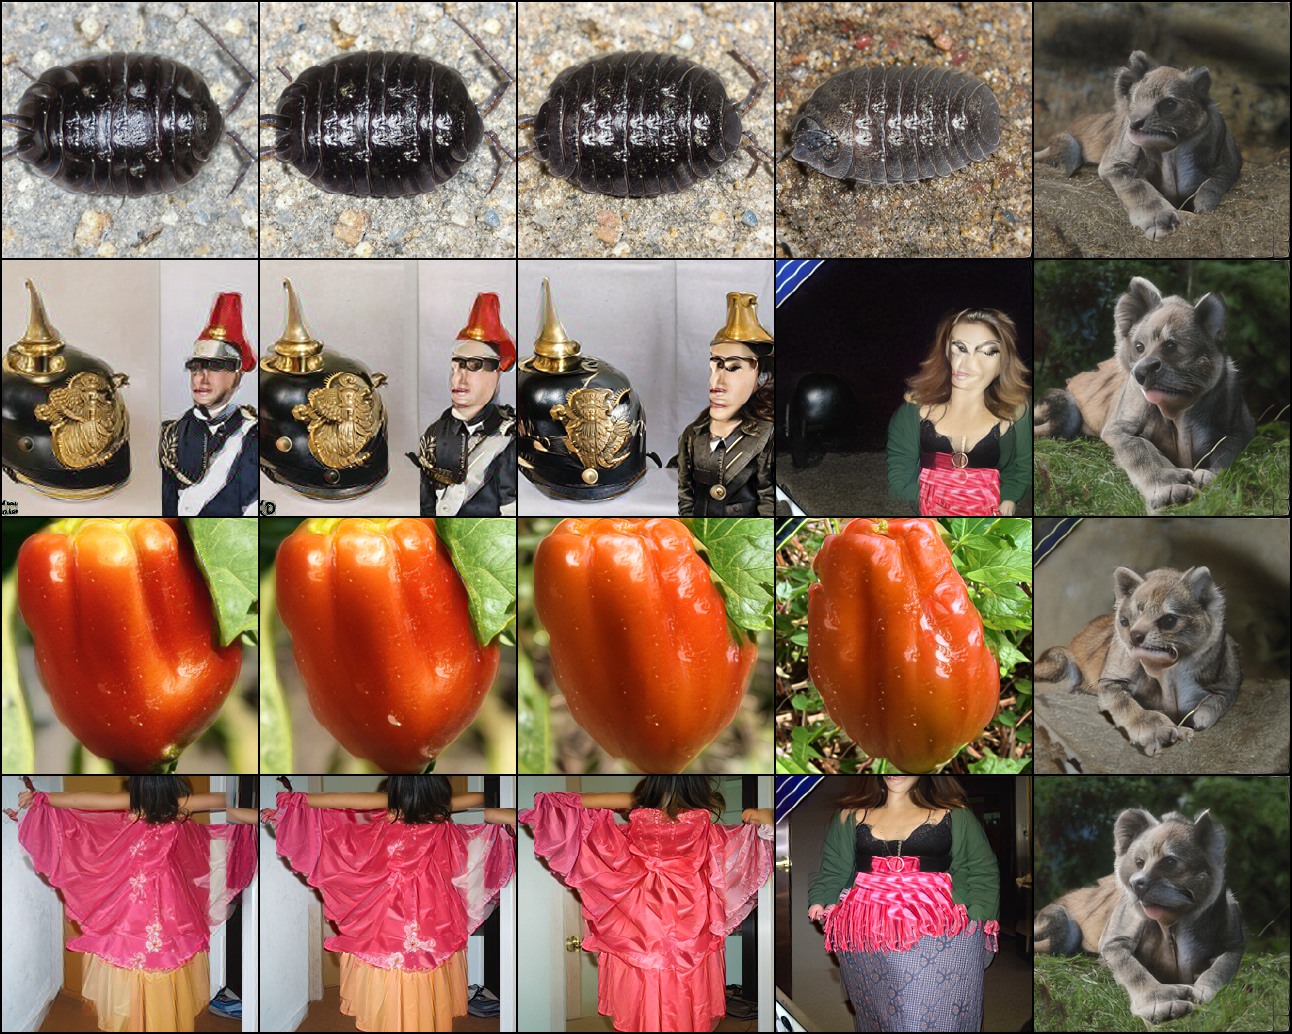
\includegraphics[width=0.45\linewidth]{imgs/GANcollapse.png}
    \captionof{figure}{Illustration of GAN collapse under a vanilla adversarial loss. Rows show different tuples of clean image, latent $z_1$, class label, and noise; columns show decreasing time values. The model remains reasonable in the high-signal region but can collapse at low time values.}
    \label{fig:gancollapse}
\end{center}

Figure~\ref{fig:gradnorm} compares the gradient norms of the GAN loss and the CrossFlow loss across time. The GAN gradient remains relatively stable, whereas the CrossFlow gradient varies with time, motivating a time-dependent adversarial weight.

\begin{center}
    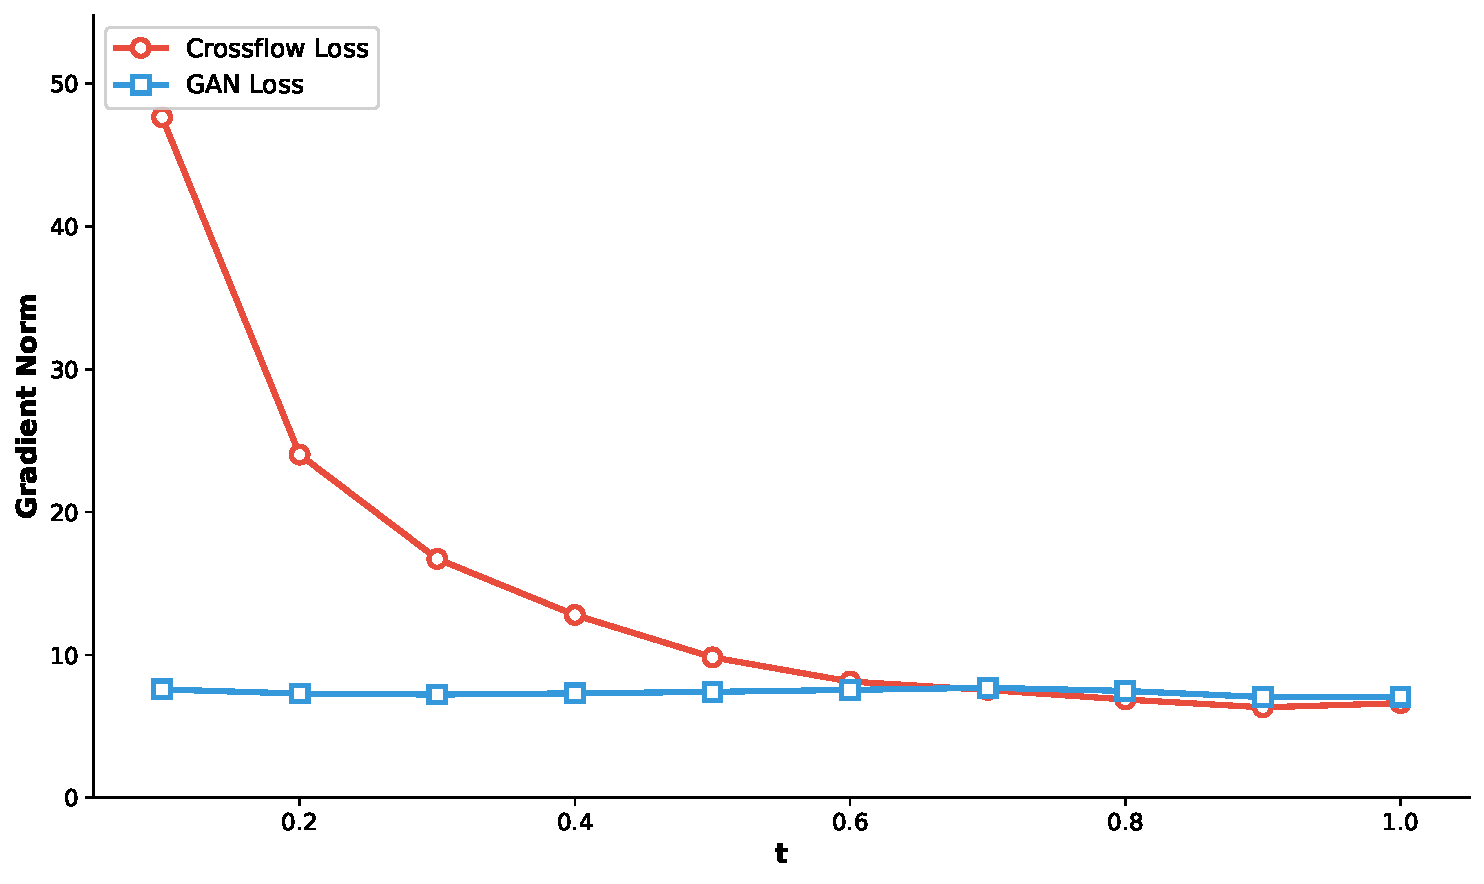
\includegraphics[width=0.5\linewidth]{imgs/plot_gradnorm.pdf}
    \captionof{figure}{Gradient norms of the GAN loss and CrossFlow loss across time, averaged over 204,800 training samples. The mismatch in relative gradient magnitude motivates weighting the adversarial loss by time.}
    \label{fig:gradnorm}
\end{center}

We therefore weight the generator loss by $w(t)$. We experiment with $w(t)=1-t$, $(1-t)^2$, and $(1-t)^4$, and use $(1-t)^2$ in the main experiments. Figure~\ref{fig:gan_weight} shows the resulting FID trajectories: too small a weight leads to weak adversarial refinement, while too large a weight can cause collapse.

\section{Additional Details on the CrossFlow Design Space}
\label{app:crossflow_design_space}

This appendix gives the details behind Sec.~\ref{sec:crossflow_design_space}. The purpose of the toy experiment is diagnostic: it checks which mathematical choices give a usable one-step map from noisy latents to images. It is not used as a main benchmark.

The CrossFlow objective Eq.~\eqref{eq:crossflow_loss_family} contains several time-dependent coefficients. The noise schedule $\alpha,\beta$ defines the latent probability path, while $\phi,\lambda,\gamma$ determine the one-step statistic and its induced training residual. The natural design order is:
\[
\text{choose } \phi(r)
\quad\Longrightarrow\quad
\text{choose } \lambda(t,r)
\quad\Longrightarrow\quad
\text{derive } \gamma(t,r).
\]
Indeed, the velocity-cancellation condition Eq.~\eqref{eq:cancel_v} gives
\begin{equation}
\gamma(t,r)\lambda(t,r)
=
1-\frac{\phi(r)}{\beta(t)}.
\label{eq:app_cancel_v}
\end{equation}
Therefore, once $\phi$ and $\lambda$ are chosen, the original coefficient $\gamma$ is determined by
\begin{equation}
\gamma(t,r)
=
\frac{1-\phi(r)/\beta(t)}{\lambda(t,r)}.
\label{eq:app_gamma_from_phi_lambda}
\end{equation}

When $\phi(r)\neq0$, we can divide the residual by $\phi(r)$. We denote the divided coefficient by
\begin{equation}
\tilde{\gamma}(t,r)
:=
\frac{\gamma(t,r)}{\phi(r)}
=
\frac{1}{\lambda(t,r)}
\left(
\frac{1}{\phi(r)}
-
\frac{1}{\beta(t)}
\right).
\label{eq:app_tilde_gamma_from_phi_lambda}
\end{equation}
Thus, after Observation~1, the practical design space is most clearly discussed in terms of $\tilde{\gamma}$, while the original coefficient is always recovered as
\begin{equation}
\gamma(t,r)=\phi(r)\tilde{\gamma}(t,r).
\label{eq:app_gamma_recover}
\end{equation}

We use a Swiss-roll toy problem as a diagnostic. All variants use the same MLP, the same fixed encoder, the same detached directional derivative, the same paired-data conditional velocity, and 800 training steps. Lower sliced Wasserstein distance (SWD) is better. The toy implementation uses the reverse time convention, where $t=0$ is noise and $t=1$ is the clean latent; for readability, the formulas below are written in the paper convention.

\begin{table}[t]
\centering
\caption{Swiss-roll diagnostic for the main design choices. In O2 and O3, the variants are written in terms of the divided coefficient $\tilde{\gamma}=\gamma/\phi$. The original coefficient is $\gamma=\phi\tilde{\gamma}$. The cosine rows use $\alpha^2+\beta^2=1$; all other rows use the linear schedule. Lower SWD is better.}
\label{tab:design_questions_main}
\small
\resizebox{\linewidth}{!}{%
\begin{tabular}{l l c}
\hline
Observation & Variant & SWD $\downarrow$ \\
\hline
O1 & $\phi(r)=\beta(r)$, $\lambda=1$, hence $\gamma(t,r)=1-\frac{\beta(r)}{\beta(t)}$ and $\tilde{\gamma}(t,r)=\frac{1}{\beta(r)}-\frac{1}{\beta(t)}$ & $0.0087$ \\
O1 & $\phi=0$, no boundary condition & $0.4483$ \\
O1 & $\phi=0$, clean boundary only & $0.3938$ \\
\hline
O2 & $\tilde{\gamma}(t,r)=\frac{1}{\beta(t)}$, never zero & $0.2775$ \\
O2 & $\tilde{\gamma}(t,r)=\frac{1}{\beta(r)}-\frac{1}{\beta(t)}$, diagonal zero $\tilde{\gamma}(t,t)=0$ & $0.0087$ \\
O2 & $\tilde{\gamma}_\delta(t,r)=\frac{1}{\beta(r+0.1)}-\frac{1}{\beta(t)}$, shifted zero $\tilde{\gamma}_\delta(t,t-0.1)=0$ & $0.0169$ \\
O2 & $\tilde{\gamma}_\delta(t,r)=\frac{1}{\beta(r+0.2)}-\frac{1}{\beta(t)}$, shifted zero $\tilde{\gamma}_\delta(t,t-0.2)=0$ & $0.0455$ \\
\hline
O3 & linear schedule, inverse-$\beta$ $\tilde{\gamma}$, matched & $0.0087$ \\
O3 & linear schedule, cosine-matched $\tilde{\gamma}(t,r)=\cot\frac{\pi r}{2}-\cot\frac{\pi t}{2}$, not matched & $0.3829$ \\
O3 & cosine schedule, inverse-$\beta$ $\tilde{\gamma}$, not matched & $0.0125$ \\
O3 & cosine schedule, $\tilde{\gamma}(t,r)=\cot\frac{\pi r}{2}-\cot\frac{\pi t}{2}$, matched & $0.0094$ \\
\hline
\end{tabular}%
}
\end{table}

\paragraph{Observation 1: choose $\phi(r)\neq0$ so the loss contains the data term.}
The first question is whether we can set $\phi(r)$ to the constant zero function. If $\phi(r)=0$, Eq.~\eqref{eq:app_cancel_v} gives
\begin{equation}
\gamma(t,r)\lambda(t,r)=1.
\end{equation}
In this case, the image-valued data term disappears from the residual:
\begin{equation}
\mathcal L_{\phi=0}
=
\mathbb E
\left\|
\partial_t\gamma(t,r)F_\theta(z_t,t,r)
+
\gamma(t,r)\frac{\mathrm d F_\theta}{\mathrm dt}
\right\|_2^2 .
\label{eq:cons_branch}
\end{equation}
For example, with $\gamma(t,r)=1$, the loss only asks the prediction to remain constant along the latent trajectory. It does not specify which image should be predicted. Therefore, the $\phi=0$ branch needs an additional boundary loss, similar to consistency models. The toy experiment confirms this behavior: with no boundary, the model is essentially unanchored; with only a clean boundary, generation from noise is still poor. In contrast, the branch $\phi(r)\neq0$ performs much better because the residual itself contains the image-valued data term.

When $\phi(r)=0$, Eq.~\eqref{eq:app_cancel_v} gives $\gamma(t,r)\lambda(t,r)=1$, and the one-space statistic becomes
\begin{equation}
Z(z_t, t, r; \lambda, \gamma)
=
\lambda(t, r)
\left(
z_t
+
\int_{t}^{r} v(z_\tau,\tau)\,\mathrm d\tau
\right),
\label{eq:consistency_statistic}
\end{equation}
which is a scaled consistency-model statistic. This branch asks the prediction to remain consistent along the probability-flow trajectory. Its cross-space loss is
\begin{equation}
\mathbb E_{x_0,\epsilon,t,r}
\left\|
\partial_t\gamma(t,r)F_\theta(z_t,t,r)
+
\gamma(t,r)\frac{\mathrm dF_\theta}{\mathrm dt}
\right\|_2^2 .
\label{eq:consistency_like_loss}
\end{equation}
For $\gamma(t,r)=1$, this reduces to the standard consistency-style constraint
\begin{equation}
\mathbb E_{x_0,\epsilon,t,r}
\left\|
\frac{\mathrm dF_\theta}{\mathrm dt}
\right\|_2^2 .
\label{eq:standard_consistency_loss}
\end{equation}
The constraint keeps the image prediction unchanged along the trajectory, but it does not identify which image should be predicted. A trivial constant output can satisfy it. This branch therefore needs an additional reconstruction boundary,
\begin{equation}
\mathbb E_{x_0\sim p_{\mathrm{data}}}
\left\|
F_\theta(\mathcal E(x_0),0,0)-x_0
\right\|_2^2 .
\label{eq:reconstruction_boundary}
\end{equation}
This makes the branch a minimal cross-space consistency baseline: the flow loss enforces invariance, while the boundary loss defines the invariant prediction.

There is also a boundary subtlety. Two-point consistency models in one space use the noisy-state boundary $Z(z_t,t,t)=\gamma(t,t)z_t$. In cross-space generation, this boundary has no direct analogue because $z_t$ is latent-valued but the desired output is image-valued. We keep this branch as a meaningful baseline, but not as the preferred CrossFlow objective.

We therefore use the branch $\phi(r)\neq0$. Since $\phi$ depends only on $r$, dividing the residual by $\phi(r)$ does not introduce additional $t$-derivative terms. Using $\tilde{\gamma}=\gamma/\phi$, the divided residual can be written as
\begin{equation}
\mathcal L_{\phi\neq0}
=
\mathbb E
\Bigg\|
\partial_t\tilde{\gamma}(t,r)F_\theta(z_t,t,r)
+
\tilde{\gamma}(t,r)\frac{\mathrm dF_\theta}{\mathrm dt}
-
\frac{\dot\beta(t)}{\beta(t)^2}
\left(
\alpha(t)-\dot\alpha(t)\frac{\beta(t)}{\dot\beta(t)}
\right)x_0
\Bigg\|_2^2 .
\label{eq:neq_loss}
\end{equation}
Multiplying the whole residual by $-1$ gives an equivalent squared loss; Eq.~\eqref{eq:neq_loss} uses the sign convention induced by $\tilde{\gamma}=\gamma/\phi$. After this simplification, the remaining design questions are how to choose $\lambda$ so that the resulting $\tilde{\gamma}$ has useful zeros, and how to match $\tilde{\gamma}$ to the noise schedule.

\paragraph{Observation 2: choose $\lambda$ so the resulting $\tilde{\gamma}$ has diagonal reconstruction anchors.}
The second question is how to choose $\lambda(t,r)$ after fixing a nonzero $\phi(r)$. From Eq.~\eqref{eq:app_tilde_gamma_from_phi_lambda},
\begin{equation}
\tilde{\gamma}(t,r)
=
\frac{1}{\lambda(t,r)}
\left(
\frac{1}{\phi(r)}
-
\frac{1}{\beta(t)}
\right).
\label{eq:app_tilde_gamma_after_lambda}
\end{equation}
Since $\tilde{\gamma}(t,r)$ multiplies $\mathrm dF_\theta/\mathrm dt$ in Eq.~\eqref{eq:neq_loss}, the derivative term vanishes wherever $\tilde{\gamma}(t,r)=0$. At such points, Eq.~\eqref{eq:neq_loss} reduces to
\begin{equation}
\mathbb E
\Bigg\|
\partial_t\tilde{\gamma}(t,r)F_\theta(z_t,t,r)
-
\frac{\dot\beta(t)}{\beta(t)^2}
\left(
\alpha(t)-\dot\alpha(t)\frac{\beta(t)}{\dot\beta(t)}
\right)x_0
\Bigg\|_2^2 .
\label{eq:recon_loss}
\end{equation}
Thus, a zero of $\tilde{\gamma}$ turns the CrossFlow residual into a reconstruction-type loss.

The most natural choice is to place this zero on the diagonal $r=t$. If $\lambda(t,r)$ is finite and nonzero, then Eq.~\eqref{eq:app_tilde_gamma_after_lambda} gives
\begin{equation}
\tilde{\gamma}(t,t)=0
\quad\Longleftrightarrow\quad
\phi(t)=\beta(t).
\label{eq:app_diagonal_phi_condition}
\end{equation}
Therefore, the simplest diagonal-anchor construction is
\begin{equation}
\phi(r)=\beta(r),
\qquad
\lambda(t,r)=1.
\label{eq:app_simple_phi_lambda}
\end{equation}
Substituting Eq.~\eqref{eq:app_simple_phi_lambda} into Eq.~\eqref{eq:app_gamma_from_phi_lambda} gives the original statistic coefficient
\begin{equation}
\gamma(t,r)
=
1-\frac{\beta(r)}{\beta(t)},
\label{eq:app_original_gamma_main}
\end{equation}
and the divided coefficient
\begin{equation}
\tilde{\gamma}(t,r)
=
\frac{\gamma(t,r)}{\phi(r)}
=
\frac{1}{\beta(r)}
-
\frac{1}{\beta(t)} .
\label{eq:gamma_inv}
\end{equation}

The toy results show why the diagonal zero matters. A simple nonzero choice, such as $\tilde{\gamma}(t,r)=1/\beta(t)$, performs poorly because the derivative term is always present and the objective never becomes a pure reconstruction anchor. Shifted-zero variants also create reconstruction anchors, but the anchors are moved away from the natural pair $(t,t)$. Their performance degrades as the shift grows. We therefore use the diagonal condition
\begin{equation}
\tilde{\gamma}(t,t)=0,
\label{eq:diagonal_zero_condition}
\end{equation}
which gives a direct reconstruction anchor at every noise level and keeps the objective easy to interpret.

\paragraph{Observation 3: choose $\phi$ and $\lambda$ jointly with the noise schedule so $\tilde{\gamma}$ has the correct scale.}
Eq.~\eqref{eq:recon_loss} shows that, when $\tilde{\gamma}(t,t)=0$, the diagonal residual becomes a reconstruction loss. However, it reconstructs $x_0$ itself only if the coefficient of $F_\theta$ matches the coefficient of $x_0$. This requires
\begin{equation}
\partial_t\tilde{\gamma}(t,t)
=
\frac{\dot\beta(t)}{\beta(t)^2}
\left(
\alpha(t)-\dot\alpha(t)\frac{\beta(t)}{\dot\beta(t)}
\right).
\label{eq:diagonal_scale_condition}
\end{equation}
Otherwise, the model is asked to fit a scaled version of $x_0$, which makes the supervision less direct.

A convenient construction is to choose a scalar function $g$ and set
\begin{equation}
\tilde{\gamma}(t,r)
=
g(r)-g(t),
\label{eq:app_tilde_gamma_g_difference}
\end{equation}
where
\begin{equation}
g'(t)
=
-\frac{\dot\beta(t)}{\beta(t)^2}
\left(
\alpha(t)-\dot\alpha(t)\frac{\beta(t)}{\dot\beta(t)}
\right).
\label{eq:schedule_matched_gamma}
\end{equation}
Then $\tilde{\gamma}(t,t)=0$, and
\begin{equation}
\partial_t\tilde{\gamma}(t,t)
=
-g'(t)
=
\frac{\dot\beta(t)}{\beta(t)^2}
\left(
\alpha(t)-\dot\alpha(t)\frac{\beta(t)}{\dot\beta(t)}
\right),
\end{equation}
so Eq.~\eqref{eq:diagonal_scale_condition} is satisfied.

This desired $\tilde{\gamma}$ can be implemented in the original design order. First choose
\begin{equation}
\phi(r)=\frac{1}{g(r)} .
\label{eq:app_phi_from_g}
\end{equation}
Then choose
\begin{equation}
\lambda(t,r)
=
\frac{
g(r)-\frac{1}{\beta(t)}
}{
g(r)-g(t)
}.
\label{eq:app_lambda_from_g}
\end{equation}
Substituting Eqs.~\eqref{eq:app_phi_from_g} and~\eqref{eq:app_lambda_from_g} into Eq.~\eqref{eq:app_tilde_gamma_from_phi_lambda} gives
\begin{equation}
\begin{aligned}
\tilde{\gamma}(t,r)
&=
\frac{1}{\lambda(t,r)}
\left(
\frac{1}{\phi(r)}
-
\frac{1}{\beta(t)}
\right) \\
&=
\frac{g(r)-g(t)}
{g(r)-\frac{1}{\beta(t)}}
\left(
g(r)
-
\frac{1}{\beta(t)}
\right) \\
&=
g(r)-g(t).
\end{aligned}
\label{eq:app_tilde_gamma_recovered}
\end{equation}
The original coefficient is then
\begin{equation}
\gamma(t,r)
=
\phi(r)\tilde{\gamma}(t,r)
=
1-\frac{g(t)}{g(r)} .
\label{eq:app_original_gamma_from_g}
\end{equation}

For the linear schedule used in our main experiments, Eq.~\eqref{eq:schedule_matched_gamma} gives
\begin{equation}
g(t)=\frac{1}{\beta(t)} .
\end{equation}
Therefore,
\begin{equation}
\phi(r)=\beta(r),
\qquad
\lambda(t,r)=1,
\qquad
\gamma(t,r)=1-\frac{\beta(r)}{\beta(t)},
\qquad
\tilde{\gamma}(t,r)=\frac{1}{\beta(r)}-\frac{1}{\beta(t)} .
\end{equation}
This recovers the simple CrossFlow construction. In practice, we clip the endpoint singularity for numerical stability.

For schedules that do not satisfy $\alpha+\beta=1$, inverse-$\beta$ is no longer automatically schedule-matched. For example, for the cosine schedule
\begin{equation}
\alpha(t)=\cos\frac{\pi t}{2},
\qquad
\beta(t)=\sin\frac{\pi t}{2},
\qquad
\alpha(t)^2+\beta(t)^2=1,
\end{equation}
Eq.~\eqref{eq:schedule_matched_gamma} gives
\begin{equation}
g(t)=\cot\frac{\pi t}{2}.
\end{equation}
A schedule-matched construction is therefore
\begin{equation}
\phi(r)=\tan\frac{\pi r}{2},
\qquad
\lambda(t,r)
=
\frac{
\cot\frac{\pi r}{2}
-
\frac{1}{\sin(\pi t/2)}
}{
\cot\frac{\pi r}{2}
-
\cot\frac{\pi t}{2}
},
\end{equation}
which yields
\begin{equation}
\tilde{\gamma}_{\cos}(t,r)
=
\cot\frac{\pi r}{2}
-
\cot\frac{\pi t}{2}.
\label{eq:gamma_cos}
\end{equation}
In the Swiss-roll diagnostic, this schedule-matched cosine choice improves over raw inverse-$\beta$ and gives the best cosine-schedule result.

Overall, the design rule is simple. First choose $\phi(r)\neq0$ so that the residual contains an image-valued target. Then choose $\lambda(t,r)$ to satisfy the desired endpoint behavior and to place reconstruction anchors at useful locations. Finally, $\gamma$ is determined by Eq.~\eqref{eq:app_gamma_from_phi_lambda}, and the divided residual is governed by $\tilde{\gamma}=\gamma/\phi$. For the linear schedule, this logic gives $\phi(r)=\beta(r)$, $\lambda(t,r)=1$, $\gamma(t,r)=1-\beta(r)/\beta(t)$, and $\tilde{\gamma}(t,r)=1/\beta(r)-1/\beta(t)$, with mild endpoint clipping for numerical stability.